\chapter{Arhitektura središnje pristupne točke}
U ovom se poglavlju opisuje arhitektura sustava. Opisuje se način na koji je lokalna mreža usmjerena
kroz pristupnu točku, gdje se i kako prikuplja mrežni promet te kako se prikupljeni podatci pohranjuju, vizualiziraju te u konačnici kako se s tim podatcima 
rukuje kako bi se postigla automatska detekcija. Naglasak je na odlukama o dizajnu i njihovim opravdanjima, dok se konkretna implementacija obrađuje kasnije.

\section{Pregled sustava}
Sustav je zamišljen da pretvori računalo s odgovarajućim sklopovljem u jedinstvenu točku kroz koju prolazi sav promet lokalne mreže, čime se ostvaruje potpuna 
vidljivost komunikacije između lokalnih uređaja i vanjskih odredišta. Računalo istovremeno obavlja funkciju usmjernika \engl{router}, pristupne točke, 
mrežnog senzora i vatrozida. Ovakvom tipu posla najviše odgovara računalo koje na sebi ima instaliran Linux, te iako su mogući i drugi načini oni se kroz rad
ne istražuju.

Slika \ref{fig:tok-podataka} prikazuje tok podataka kroz sustav. Sav mrežni promet prolazi kroz Zeek koji ga analizira i pohranjuje u obliku strukturiranih JSON zapisa 
u direktorij dijeljen s ostalim servisima. Tom direktoriju pristupaju dva različita podsustava za pohranu, no ne istovremeno. Prvi podsustav čini vremenski orijentirana 
baza InfluxDB, u koju podatke unosi agent Telegraf. Drugi čini dokumentno orijentirana baza Elasticsearch, u koju podatke unosi agent Filebeat. Oba podsustava kao zajedničko 
vizualizacijsko sučelje koriste Grafanu. Postojanje dvaju podsustava ne predstavlja produkcijsku konfiguraciju, nego služi njihovoj usporedbi provedenoj u poglavlju o 
evaluaciji. U produkcijskom bi se okruženju odabrao jedan od njih, ovisno o potrebama korisnika i mogućnostima dostupnog sklopovlja.

\begin{figure}[ht]
  \centering
  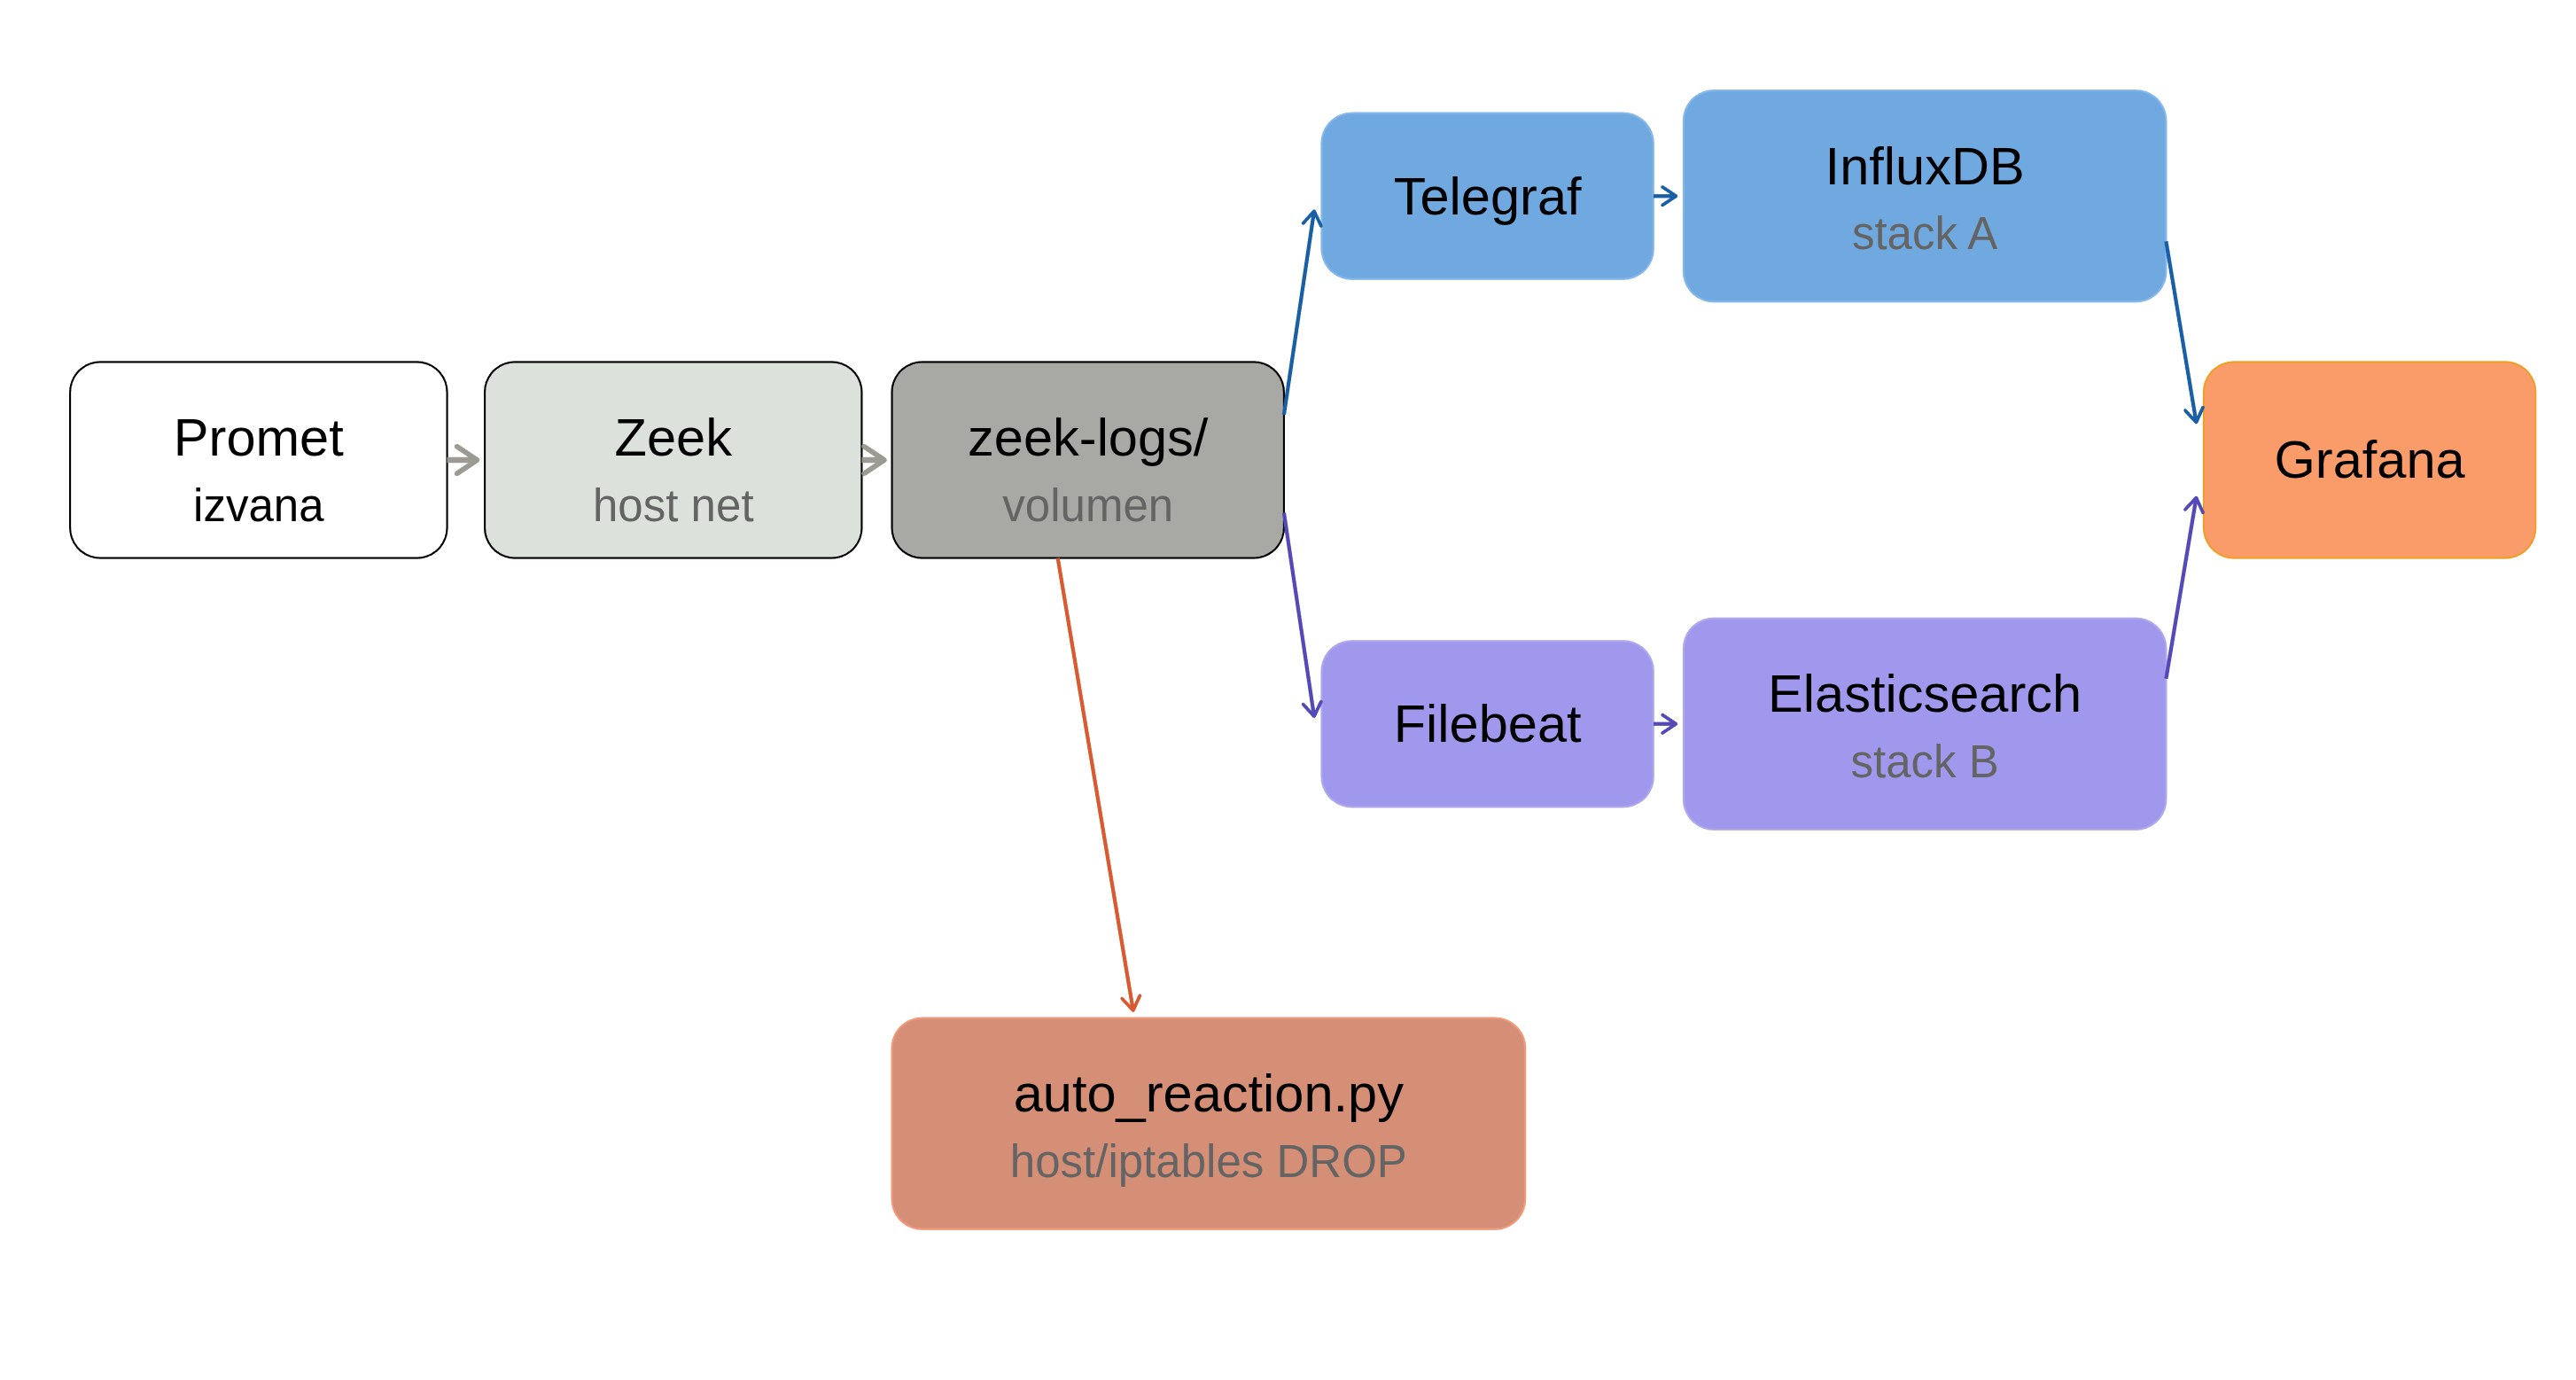
\includegraphics[width=0.95\textwidth]{slike/tok_podataka_dual_stack_custom.png}
  \caption{Prikaz toka podataka kroz sustav}
  \label{fig:tok-podataka}
\end{figure}

Svi navedeni servisi izvode se u Docker kontejnerima, čime se postiže ponovljivost i prenosivost okruženja te jednostavnost pri postavljanju \cite{docker_docs}. 
Jedina je iznimka skripta za automatsku reakciju, koja se izvodi izravno na računalu domaćinu jer mijenja njegova vatrozidna pravila, o čemu je više riječi u kasnijem odjeljku.

\section{Usmjeravanje, NAT i pristupna točka}
Mrežna topologija sustava prikazana je na slici \ref{fig:topologija}. 

\begin{figure}[h]
  \centering
  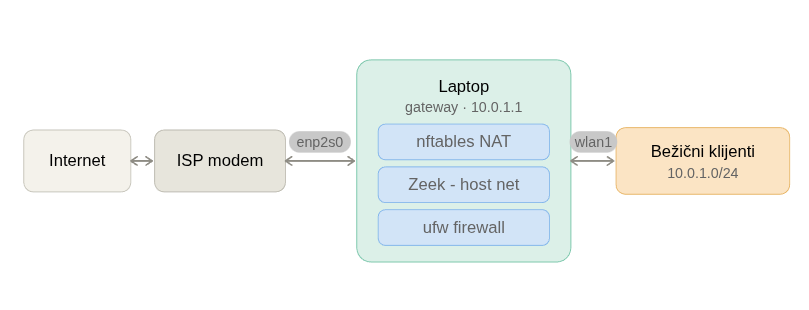
\includegraphics[width=0.95\textwidth]{slike/mrezna_topologija_custom.png}
  \caption{Mrežna topologija}
  \label{fig:topologija}
\end{figure}
Računalo koje objedinjuje uloge prikazane na slici \ref{fig:topologija} mora posjedovati barem dva mrežna sučelja. Jedno je žično sučelje povezano prema 
pružatelju internetskih usluga \engl{Internet Service Provider, ISP} i služi kao izlaz prema internetu. Drugo je bežično sučelje u ulozi pristupne točke, na 
koje se povezuju ostali uređaji lokalne mreže. Bežično se povezivanje moglo iskoristiti i za izlaz prema internetu, no žična je veza u pravilu stabilnija. Konkretni 
nazivi sučelja i pripadna konfiguracija iznose se u poglavlju o implementaciji.

Lokalni uređaji dobivaju adrese iz privatnog adresnog raspona \texttt{10.0.1.0/24}, u kojem računalo s ulogom usmjernika ima adresu \texttt{10.0.1.1}, u skladu s rasponima 
rezerviranima za privatne mreže \cite{rfc1918}. Bežično sučelje u ulogu pristupne točke postavlja alat \texttt{hostapd}, dok mrežne parametre klijentima dodjeljuje 
alat \texttt{dnsmasq} u ulozi DHCP poslužitelja.

Budući da lokalni uređaji vanjskim mrežama pristupaju isključivo preko ovog računala, sav promet između njih i vanjskih odredišta nužno prolazi kroz jednu točku, čime se 
ostvaruje potpuna vidljivost prometa nužna za analizu komunikacijskih obrazaca. Kako lokalni uređaji dijele jednu javnu adresu domaćina, na izlaznom se sučelju provodi 
prevođenje mrežnih adresa \engl{Network Address Translation, NAT}.

Upravljanje vatrozidom na računalu temelji se na dva alata, \texttt{nftables} i \texttt{ufw}. Oba djeluju nad istom pozadinskom implementacijom.
Na suvremenim se distribucijama i \texttt{ufw} izvodi kroz \texttt{nftables}, a starije \texttt{iptables} naredbe prevode se posredstvom sloja
\texttt{iptables-nft}. \texttt{nftables} je zapravo jedini pozadinski mehanizam koji se koristi, dok se naredbe ostalih alata prevode kroz \texttt{nft}.

Vatrozid \texttt{ufw} \engl{Uncomplicated Firewall} provodi pravila filtriranja izravno na domaćinu. Zadana je politika odbacivanje svog prometa, pa se 
rad pristupne točke mora izrijekom dopustiti minimalnim skupom pravila. Posljedica je da domaćin neželjeni dolazni internetski promet odbacuje već na temelju zadane 
politike, neovisno o ostalim slojevima. Konkretna se pravila iznose u poglavlju o implementaciji.

\section{Praćenje i zapisivanje prometa Zeekom}
Nadzorni sloj čini Zeek, kojem je omogućen pristup bežičnom sučelju radi praćenja prometa. Za razliku od ostalih servisa, Zeek se ne izvodi u izoliranoj kontejnerskoj 
mreži, nego koristi mrežu domaćina \engl{host network mode}, jer mora izravno pristupiti fizičkom sučelju radi osluškivanja prometa. Iako mu dodijeljene ovlasti tehnički 
dopuštaju i slanje paketa, Zeek po svojoj namjeni promet isključivo čita i ne generira ga, pa je njegova uloga u praćenju pasivna. Pojedinosti o ovlastima i načinu izvođenja 
iznose se u poglavlju o implementaciji.

Nadalje, odabir bežičnog sučelja kao mjesta praćenja nije proizvoljan. Praćenjem prije prevođenja adresa izvorišne i odredišne adrese ostaju nepromijenjene, čime se zadržava 
atribucija prometa po pojedinom uređaju, što je nužno za smislenu analizu. Nije isto ako stolno računalo ili pametni hladnjak pokreću SSH i FTP veze.

Zeek prepoznaje i prati mnoštvo mrežnih protokola te o njihovoj aktivnosti vodi strukturirane zapise koje razvrstava u zasebne datoteke prema vrsti zabilježene
aktivnosti i pohranjuje te zapise u direktorij \texttt{zeek-logs}. Među njima su, primjerice, \texttt{conn.log, dns.log, dhcp.log, http.log, ssh.log, files.log, quic.log i notice.log}. 
Većina je datoteka vezana uz pojedini protokol, dok pojedini zapisi bilježe izvedene događaje neovisno o protokolu. Najvažnija takva datoteka je \texttt{notice.log}, u koju Zeek upisuje 
upozorenja na temelju kojih se pokreće automatska reakcija opisana kasnije u ovom poglavlju. Sljedeći važan zapis je \texttt{conn.log} u kojem se nalazi zapis preostalog prometa poput TCP, UDP, ICMP.
Kratki opis ostalih zapisa nalazi se u tablici \ref{tab:tablica-datoteka}.

\begin{table}[htb]
  \centering
  \begin{tabular}{l|p{12cm}}
      \hline
      Naziv datoteke & Opis \\
      \hline
      \texttt{dns.log} & zapisuje sve DNS upite \\
      \texttt{dhcp.log} & zapisuje klijente te informacije o njihovim IP adresama, MAC-ovima, nazivima \\
      \texttt{http.log} & zapisuje sve HTTP zahtjeve zato što su nešifrirani i bogati metapodatcima za razliku od HTTPS zahtjeva \\
      \texttt{ssh.log} & zapisuje sve SSH veze \\
      \texttt{files.log} & sve datoteke koje su prenesene kroz nadzirano sučelje \\
      \texttt{quic.log} & zapis o brzim UDP vezama \engl{Quick UDP Internet Connections} \\
      \hline
  \end{tabular}
  \caption{Nazivi i opisi datoteka u \texttt{zeek-logs}.}
  \label{tab:tablica-datoteka}
\end{table}

Zapisi se generiraju u JSON formatu, čime se omogućuje njihovo izravno strojno čitanje. Time direktorij \texttt{zeek-logs} postaje
jedinstvena predajna točka prema podsustavima za pohranu, opisanima u nastavku.


\section{Tok podataka i pohrana}
Zeekovi zapisi iz direktorija \texttt{zeek-logs} su ulazna točka za pohranu, kako je prikazano na slici \ref{fig:tok-podataka}. Taj je direktorij u Zeekovom
kontejneru montiran s pravom pisanja, a u agente za prikupljanje isključivo s pravom čitanja. Time se prikupljanje odvaja od pohrane.

Nad istim se zapisima ispituju dva podsustava za pohranu. Prvi čini agent Telegraf, koji Zeekove JSON zapise upisuje u vremenski orijentiranu bazu
InfluxDB. Drugi čini agent Filebeat, koji iste zapise prosljeđuje u dokumentno orijentiranu bazu Elasticsearch. Uloge i svojstva pojedinih alata podrobnije su
opisani u prethodnom poglavlju o teorijskim osnovama.

Ta dva podsustava nisu predviđena za istovremeni rad. Definirani su u zasebnim konfiguracijama, od kojih svaka sadrži vlastiti senzor i vlastitu instancu Grafane, 
pa se u danom trenutku izvodi isključivo jedan. Razdvajanje ima dva cilja. Prvo, izolacija sprječava da trošenje resursa jednog podsustava iskrivi mjerenja drugoga, 
što je preduvjet poštene usporedbe provedene u poglavlju o evaluaciji. Drugo, budući da obje konfiguracije kao ulaz koriste isti skup Zeekovih zapisa istoga formata, 
razlike u rezultatima moguće je pripisati isključivo pozadinskoj bazi, a ne ulaznim podatcima.

\section{Prepoznavanje i automatska reakcija}
Prepoznavanje i automatska reakcija odvijaju se u dva koraka. Najprije Zeek prepoznaje kada je neka veza sumnjiva. Podrazumijevano Zeek ne prepoznaje maliciozne veze, 
no dolazi s većim brojem gotovih detektora i okvira koje je moguće uključiti i prilagoditi. Uz njih se detekcijska logika proširuje i vlastitim pravilima opisanima 
Zeekovim skriptnim jezikom, kao i indikatorima kompromitacije \engl{Indicators of Compromise, IoC} koji se zadaju kao popis adresa neovisan o samoj logici. Kada Zeek 
prepozna takav događaj, upisuje upozorenje u \texttt{notice.log}.

Na to se nadovezuje drugi korak, skripta za automatsku reakciju \texttt{auto\_reaction.py}. Ona prati novoupisana upozorenja i na temelju njih blokira izvorišne adrese. 
Skripta se izvodi s administratorskim ovlastima jer mijenja vatrozidna pravila računala domaćina.

Blokiranje je izvedeno preko skupa \engl{set} koji sadrži blokirane adrese, a zasebni lanci vatrozida odbacuju sav promet čija se izvorišna adresa nalazi u tom skupu. 
Ti su lanci postavljeni na viši prioritet od zadanih \texttt{ufw} lanaca, pa odbacivanje stupa na snagu prije nego što ostala pravila propuste vezu. Adrese usmjernika i 
lokalnog domaćina izuzete su popisom dopuštenih adresa \engl{whitelist} kako bi se spriječilo blokiranje vlastite infrastrukture.

Nadalje, potrebno je istaknuti i ograničenje autorovog rješenja, odnosno reakcija se temelji na izvorišnoj adresi iz zapisa upozorenja. U slučaju lažiranja izvorišne adrese
\engl{spoofing} skripta blokira adresu navedenu u zapisu, koja ne mora odgovarati stvarnom napadaču. To znači da napadač može lažirati adresu
legitimnog korisnika odnosno uređaja. Kako bi se to izbjeglo predlaže se stalno ažuriranje popisa dopuštenih adresa uređajima kojima se vjeruje kao i dodjela 
statičkih adresa uređajima od povjerenja.

Svaki element prethodno navedenog skupa nosi vremensko ograničenje \engl{timeout} kojim upravlja jezgra operacijskog sustava, pa se pravilo uklanja automatski 
nakon isteka, bez ikakve intervencije korisnika ili skripte. Time se izbjegava slabost izvedbe zasnovane na izravnim pravilima. Ukratko to znači da nasilni 
prekid skripte (signalom \texttt{SIGKILL}, nedostatkom memorije ili gubitkom napajanja) ne ostavlja zaostala pravila jer ona ionako isteknu sama.